%==================================================================================================
\section{Equações Governantes da Dinâmica dos Sólidos} \label{EGDS}
%==================================================================================================

O estudo dos elementos sólidos baseia-se na determinação de parâmetros referentes à elementos estruturais, tais como esforços internos e deslocamentos, ou tensões e deformações. Em alguns casos particulares isso pode ser obtido através da simples consideração das relações de equilíbrio, de compatibilidade e constitutivas. Entretanto, em vários outros casos, pode ser necessário o uso de algumas técnicas, como o uso dos princípios variacionais, que serão devidamente descritos na presente seção.

Para se utilizar desses princípios, deve-se primeiramente definir o conceito de energia total ($\Pi$) de um sistema, que pode ser entendido como a soma de todas as parcelas relevantes ao problema. Em casos mais comuns de problemas envolvendo elementos sólidos, tem-se a consideração de uma parcela de energia devida às forças externas atuantes no corpo ($\mathbb{P}$), energia de deformação ($\mathbb{U}$) e energia cinética ($\mathbb{K}$). Dessa forma:

\begin{equation}
    \Pi=\mathbb{P}+\mathbb{U}+\mathbb{K}\text{.}
\end{equation}

Nesse sentido, busca-se encontrar uma configuração que esteja em equilíbrio estável. Dessa forma postula-se o primeiro teorema variacional, que aponta que, para se obter o equilíbrio em um sólido sujeito a forças externas conservativas, a primeira variação da energia total deve ser nula para qualquer variação admissível, ou seja:

\begin{equation}
    \delta^{(1)}\Pi=0\forall\delta\BB{u}|\delta\BB{u}=\BB{0}\text{ em }\Gamma_D\text{,}
\end{equation}

\noindent em que $\Gamma_D$ é a parcela da fronteira onde os deslocamentos são prescritos. Já o segundo teorema trata-se da estabilidade desse equilíbrio, onde para se atingir o equilíbrio estável a segunda variação da energia total deve ser positiva para qualquer variação admissível, ou seja:

\begin{equation}
    \delta^{(2)}\Pi>0\forall\delta\BB{u}|\delta\BB{u}=\BB{0}\text{ em }\Gamma_D\text{.}
\end{equation}

Sendo assim, primeiramente procura-se anular a primeira variação da energia total:

\begin{equation}
    \delta\Pi=\delta\mathbb{P}+\delta\mathbb{U}+\delta\mathbb{K}=0\text{,}
\end{equation}

\noindent o que leva à necessidade de se determinar a primeira variação de $\mathbb{U}$. Para isso, é necessária a consideração de um modelo constitutivo que descreva a evolução da energia de deformação em função da medida de deformação.

Na sequência serão apresentadas algumas medidas de deformação uniaxiais para fins de exemplificação, sendo as medidas de deformação multiaxiais apresentadas posteriormente na seção \ref{CCD}.

A primeira medida de deformação que pode ser observada é a denominada medida de deformação linear (ou de engenharia), que se trata de uma medida Lagrangiana, pois toma como referência a configuração inicial (ou indeformada) do elemento, e é definida como:

\begin{equation}
    \varepsilon=\frac{dy-dx}{dx}\text{,}
\end{equation}

\noindent em que $dx$ e $dy$ são os comprimentos de um trecho infinitesimal de uma barra em sua configuração inicial e atual, respectivamente (Figura \ref{fig:Barra}).

\begin{figure}[h!]
    \centering
    \caption{Desenho esquemático de uma barra submetida a tração.}
    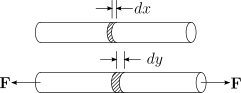
\includegraphics[width=0.45\linewidth]{Figuras/Barra.pdf}
    \\Fonte: Autoria Própria (\the\year).
    \label{fig:Barra}
\end{figure}

Outra medida de deformação Lagrangiana interessante é a medida de deformação quadrática (ou de Green-Lagrange), definida como:

\begin{equation}
    \mathbb{E}=\frac{1}{2}\frac{dy^2-dx^2}{dx^2}\text{.}
\end{equation}

Vale ressaltar que, em comparação com a medida de deformação linear, a deformação quadrática pode ser utilizada para problemas com uma deformação maior, descrevendo uma variedade maior de problemas.

Já outras medidas de deformação Eulerianas (que tomam como referência a configuração atual do elemento) tem-se a medida de deformação de Almansi:

\begin{equation}
    \mathbb{A}=\frac{1}{2}\frac{dy^2-dx^2}{dy^2}\text{,}
\end{equation}

\noindent e a medida de deformação de Hencky:

\begin{equation}
    \mathbb{H}=-\ln{\left(\frac{dx}{dy}\right)}\text{.}
\end{equation}

Assim, pode-se definir alguns modelos constitutivos que relacionarão a medida de tensão com a de deformação, ou de forma mais prática, a medida de energia específica de deformação ($u_e$) com alguma dessas duas medidas, sendo $u_e$ a energia de deformação por unidade de volume, matematicamente interpretado como a área sob a curva de tensão $\times$ deformação (Figura \ref{fig:ue}), ou seja:

\begin{equation}
    u_e=\int_0^\varepsilon{\sigma d\varepsilon}\text{.}
\end{equation}

\begin{figure}[h!]
    \centering
    \caption{Esquema de diagrama de tensão $\times$ deformação.}
    \includegraphics[width=.45\linewidth]{Figuras/ue.pdf}
    \\Fonte: Autoria Própria (\the\year).
    \label{fig:ue}
\end{figure}

Assim, destacam-se os modelos constitutivos de Hooke (Equação \ref{eq:Hooke}), de Saint-Venant-Kirchhoff (Equação \ref{eq:SVK}) e de Almasi (Equação \ref{eq:Almansi}):

\begin{subequations}
    \begin{equation}
        u_e^H=\frac{E\varepsilon^2}{2}\text{,}\label{eq:Hooke}
    \end{equation}
    \begin{equation}
        u_e^{SVK}=\frac{K\mathbb{E}^2}{2}\text{,}\label{eq:SVK}
    \end{equation}
    \begin{equation}
        u_e^{Al}=\frac{Z\mathbb{A}^2}{2}\text{,}\label{eq:Almansi}
    \end{equation}
\end{subequations}

\noindent em que $E$, $K$ e $Z$ representam o módulo de elasticidade longitudinal do material em seus respectivos modelos constitutivos.

Uma propriedade notável aponta a tensão como a conjugada energética da deformação, que, matematicamente, significa que a primeira derivada da energia específica de deformação em relação à medida de deformação é igual à tensão, ou seja:

\begin{equation}
    \der{u_e}{\varepsilon}=\sigma=E\varepsilon\text{.}
\end{equation}

%==================================================================================================
\subsection{Cinemática dos Corpos Deformáveis} \label{CCD}
%==================================================================================================

Inicialmente considere um corpo deformável, idealizado como um meio contínuo que, em sua configuração inicial é denotado por $\Omega_0$ e em sua configuração atual é denotado por $\Omega$, conforme ilustrado na Figura \ref{fig:Cont}. Para se mapear os pontos que compõem o corpo em relação a uma origem preestabelecida utiliza-se $\BB{x}$ e $\BB{y}$ para denotar as coordenadas de $\Omega_0$ e $\Omega$, respectivamente. Já para se mapear $\BB{y}$ em função de $\BB{x}$ existe uma função $\BB{f}$ tal que $\BB{y}=\BB{f}(\BB{x})$, denominada como função de mudança de configuração.

\begin{figure}[h!]
    \centering
    \caption{Configurações inicial e atual de um corpo deformável.}
    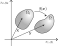
\includegraphics[width=.4\linewidth]{Figuras/Cont.pdf}
    \\Fonte: Autoria Própria (\the\year).
    \label{fig:Cont}
\end{figure}

Para um ponto $\BB{x}$ na vizinhança de $\BB{x}_0$, pode-se dizer que:

\begin{equation}
    \BB{y}(\BB{x})=\BB{f}(\BB{x}_0)+\left.\der{\BB{f}}{\BB{x}}\right|_{\BB{x}_0}\cdot d\BB{x}\text{,}
\end{equation}

\noindent em que $\BB{A}=\partial\BB{f}/\partial\BB{x}$ é o gradiente de mudança de configuração. Assim, pode-se obter uma expressão que transforme um vetor $d\BB{x}$ na configuração inicial em um vetor $d\BB{y}$ na atual:

\begin{equation}
    d\BB{y}=\BB{A}\cdot d\BB{x}\text{,}\label{eq:dyAdx}
\end{equation}

\noindent o que permite escrever o quadrado da norma de $d\BB{y}$ como:

\[
    \norm{d\BB{y}}^2=dy^2=d\BB{y}^T\cdot d\BB{y}=(\BB{A}\cdot d\BB{x})^T\cdot(\BB{A}\cdot d\BB{x})=d\BB{x}^T\cdot\BB{A}^T\cdot\BB{A}\cdot d\BB{x}
\]

Subtraindo-se $dx^2=\norm{d\BB{x}}^2$ de ambos os lados da igualdade obtém-se:

\begin{equation}
    dy^2-dx^2=d\BB{x}^T\cdot(\BB{A}^T\cdot\BB{A}-\BB{I})\cdot d\BB{x}\text{,}
    \label{eq:difdxdy}
\end{equation}

\noindent em que $\BB{I}$ é o tensor identidade de segunda ordem e $\BB{C}=\BB{A}^T\cdot\BB{A}$ é o tensor de alongamento à direita de Cauchy-Green. Dessa maneira, pode-se substituir $\BB{C}$ em \ref{eq:difdxdy} e dividir por $2dx^2$, obtendo-se:

\[
    \frac{1}{2}\frac{dy^2-dx^2}{dx^2}=\frac{1}{2}\frac{d\BB{x}^T\cdot(\BB{C}-\BB{I})\cdot d\BB{x}}{dx^2}\text{.}
\]

\noindent Tomando um versor na direção de $d\BB{x}$ ($\BB{u}=d\BB{x}/\norm{d\BB{x}}$), tem-se que:

\begin{equation}
    \frac{1}{2}\frac{dy^2-dx^2}{dx^2}=\BB{u}^T\cdot\left(\frac{1}{2}(\BB{C}-\BB{I})\right)\cdot\BB{u}\text{.}
\end{equation}

Assim, define-se o tensor de deformações de Green-Lagrange como:

\begin{equation}
    \mathbb{E}=\frac{1}{2}(\BB{C}-\BB{I})\text{,}
    \label{eq:CSD-DefGreenLagr}
\end{equation}

\noindent que se trata de uma medida de deformação objetiva, ou seja, não registra deformações em movimento de corpo rígido.

Outra medida de deformação interessante é a medida de deformação volumétrica ($\varepsilon_V$). Para isso considere o elemento infinitesimal em suas configurações inicial e atual ilustrado na Figura \ref{fig:MudVol}.

\begin{figure}[h!]
    \centering
    \caption{Mudança de volume de um elemento infinitesimal.}
    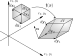
\includegraphics[width=0.5\linewidth]{Figuras/MudVol.pdf}
    \\Fonte: Autoria Própria (\the\year).
    \label{fig:MudVol}
\end{figure}

Logo o valor de $\varepsilon_V$ pode ser obtido através da relação entre o volume inicial e atual desse elemento como:

\begin{equation}
    \varepsilon_V=\frac{dV-dV_0}{dV_0}\text{.}
\end{equation}

O volume do elemento em ambas as configurações pode ser obtido por meio do produto misto dos vetores que formam o mesmo, ou seja:

\begin{subequations}
    \begin{equation}
        dV_0=d\BB{x}_1\cdot(d \BB{x}_2\times d\BB{x}_3)\text{,}
    \end{equation}
    \begin{equation}
        dV=d\BB{y}_1\cdot(d \BB{y}_2\times d\BB{y}_3)\text{,}
    \end{equation}
\end{subequations}

Conhecendo a transformação expressa em \ref{eq:dyAdx} e fazendo as devidas simplificações pode-se obter que:

\begin{equation}
    dV=\det{(\BB{A})}dV_0=JdV_0\text{,}\label{eq:RelVol}
\end{equation}

\noindent em que $J=\det{(\BB{A})}$ é o Jacobiano da mudança de configuração.

Na sequência procura-se obter uma expressão que indique a mudança de área nas diferentes configurações. Assim, considere um cilindro infinitesimal ilustrado na figura \ref{fig:Nanson}.

\begin{figure}[h!]
    \centering
    \caption{Mudança de configuração em um cilindro infinitesimal.}
    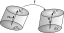
\includegraphics[width=.45\linewidth]{Figuras/Nanson.pdf}
    \\Fonte: Autoria Própria (\the\year).
    \label{fig:Nanson}
\end{figure}

Nesse contexto, a área vetorial pode ser entendida como seu valor absoluto na direção de sua normal ($d\BB{A}_0=dA_0\BB{N}$ e $d\BB{A}=dA\BB{n}$). Logo o volume do cilindro é dado pelo produto escalar da área vetorial com o vetor que define a altura do cilindro ($dV_0=d\BB{A}_0\cdot\BB{u}$ e $dV=\BB{A}\cdot\BB{v}$). Conhecendo as relações \ref{eq:dyAdx} e \ref{eq:RelVol}, pode obter que:

\begin{equation}
    \BB{n}dA=J\BB{A}^{-T}\cdot\BB{N}dA_0\text{,}\label{eq:Nanson}
\end{equation}

\noindent que é conhecida como a Equação de Nanson.

Com esse embasamento é possível apresentar os conceitos de energia nas descrições Euleriana e Lagrangiana Total. Assim, para se obter a equação do equilíbrio local de um elemento na descrição Euleriana, considere um elemento infinitesimal sujeito à ação de uma força de corpo (ou de volume) $\BB{c}$, conforme ilustrado no diagrama de corpo livre da Figura \ref{fig:CorpoLivreSolido}, que apresenta somente as forças atuantes na direção $\bhat{e}_1$.

\begin{figure}[h!]
    \centering
    \caption{Forças atuantes em um elemento infinitesimal na direção $\bhat{e}_1$.}
    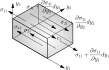
\includegraphics[width=.5\linewidth]{Figuras/CorpoLivreSolido.pdf}
    \\Fonte: Autoria Própria (\the\year).
    \label{fig:CorpoLivreSolido}
\end{figure}

Fazendo o equilíbrio das forças nessa direção tem-se:

\[
    \begin{split}
        &-\sigma_{11}dy_2dy_3-\sigma_{21}dy_1dy_3-\sigma_{31}dy_1dy_2+
        \bigpar{\sigma_{11}+\der{\sigma_{11}}{y_1}dy_1}dy_2dy_3+\\
        &\bigpar{\sigma_{21}+\der{\sigma_{21}}{y_2}dy_2}dy_1dy_3+
        \bigpar{\sigma_{31}+\der{\sigma_{31}}{y_3}dy_3}dy_1dy_2+c_1dV=\rho\ddot{y}_1dV
    \end{split}
\]

Fazendo as devidas simplificações obtém-se:

\[
    \der{\sigma_{11}}{y_1}+\der{\sigma_{21}}{y_2}+\der{\sigma_{31}}{y_3}+c_1=\rho\ddot{y}_1\text{,}
\]

\noindent que, expandindo analogamente para as demais direções, pode escrever nas notações simbólica (Equação \ref{eq:EqLocEu1}) e indicial (Equação \ref{eq:EqLocEu2}) como:

\begin{subequations}
    \begin{equation}
        \NN\cdot\tens^T+\BB{c}=\rho\ddot{\BB{y}}\text{,}\label{eq:EqLocEu1}
    \end{equation}
    \begin{equation}
        \sigma_{ij,i}+c_j=\rho\ddot{y}_j\text{,}\label{eq:EqLocEu2}
    \end{equation}
    \label{eq:EqLocEu}
\end{subequations}

\noindent as quais representam as equações do equilíbrio local na descrição Euleriana e sendo a vírgula presente no subíndice a representação de derivada na direção $i$, ou seja:

\begin{equation}
    \sigma_{ij,i}=\der{\sigma_{ij}}{y_i}\text{.}
\end{equation}

Integrando a equação \ref{eq:EqLocEu} em $\Omega$ e aplicando o teorema da divergência obtém-se:

\begin{equation}
    \int_\Gamma{\tens^T\cdot\BB{n}d\Gamma}+\int_\Omega{\BB{c}d\Omega}=\int_\Omega{\rho\ddot{\BB{y}}d\Omega}
    \text{,}
    \label{eq:EqGlobEu}
\end{equation}

\noindent onde $\Gamma=\partial\Omega$ é a fronteira do domínio de análise. Essa equação representa o equilíbrio global na descrição Euleriana.

Já em uma descrição Lagrangiana Total, será necessário transformar os termos dependentes da configuração atual para outros dependentes da configuração inicial. Assim, pode-se reescrever a Equação \ref{eq:EqGlobEu} levando em consideração as Equações \ref{eq:RelVol} e \ref{eq:Nanson}:

\begin{equation}
    \int_{\Gamma_0}{J\tens^T\cdot\BB{A}^{-T}\cdot\BB{N}d\Gamma_0}+\int_{\Omega_0}{J\BB{c}d\Omega_0}=\int_{\Omega_0}{J\rho\ddot{\BB{y}}d\Omega_0}
    \text{.}
\end{equation}

\noindent Sendo $\BB{c}^0=J\BB{c}$ as forças de corpo na configuração inicial, $\rho_0=J\rho$ a densidade inicial e $\BB{P}=J\BB{A}^{-1}\cdot\tens$ o primeiro tensor de tensões de Piola-Kirchhoff, tem-se que:

\begin{equation}
    \int_{\Gamma_0}{\BB{P}^T\cdot\BB{N}d\Gamma_0}+\int_{\Omega_0}{\BB{c}^0d\Omega_0}=\int_{\Omega_0}{\rho_0\ddot{\BB{y}}d\Omega_0}\text{,}
\end{equation}

\noindent que representa a equação do equilíbrio global na descrição Lagrangiana Total.

Retornando a integral sob a fronteira $\Gamma_0$ para $\Omega_0$ por meio do Teorema da Divergência e tomando um elemento infinitesimal de volume, pode-se obter a equação do equilíbrio local na descrição Lagrangiana Total:

\begin{subequations}
    \begin{equation}
        \NNx\cdot\BB{P}^T+\BB{c}^0=\rho_0\ddot{\BB{y}}\text{, ou}
    \end{equation}
    \begin{equation}
        P_{ij,i}+c_j^0=\rho_0\ddot{y}_j\text{.}
    \end{equation}
\end{subequations}

%==================================================================================================
\subsection{Método dos Elementos Finitos Posicional Aplicado a Elementos de Casca} \label{MEFP}
%==================================================================================================

Será exposta na presente seção a formulação para elementos de Casca baseada no Método dos Elementos Finitos Posicional, a qual seguirá uma descrição Lagrangiana Total, adotando o modelo constitutivo de Saint-Venant Kirchhoff e o tensor de deformações de Green-Lagrange ($\mathbb{E}$). Para isso, será considerado inicialmente o princípio da conservação da energia, onde as parcelas envolvidas serão aquelas devidas às forças externas ($\mathbb{P}$), de deformação ($\mathbb{U}$), cinética ($\mathbb{K}$) e a dissipação da energia total ($\mathbb{Q}$):

\begin{equation}
    \Pi_0=\mathbb{U}+\mathbb{P}+\mathbb{K}+\mathbb{Q}\text{,}
\end{equation}

\noindent sendo:

\begin{subequations}
    \begin{align}
         & \mathbb{U}=\frac{1}{2}\intDomi{S_{ij}\mathbb{E}_{ij}}\text{,}    \\
         & \mathbb{P}=-F_i^aY_i^a-\intFronti{t_iy_i^m}\text{ e}             \\
         & \mathbb{K}=\frac{1}{2}\intDomi{\rho_0\dot{y}_i\dot{y}_i}\text{,}
    \end{align}
\end{subequations}

\noindent em que $\Omega_0$ é o domínio de análise em sua configuração inicial, cuja fronteira é $\Gamma_0=\partial\Omega_0$, $F_i^a$ é uma força concentrada aplicada sobre um ponto $a$ na direção $i$, cuja posição atual é $Y_i^a$, $t_i$ é uma força distribuída sobre uma superfície média da casca ($y_i$), $\rho_0$ é a massa específica inicial do contínuo e  $S_{ij}$ é o tensor de Piola-Kirchhoff de segunda espécie, escrito como:

\begin{equation}
    S_{ij}=\script{C}_{ijkl}\mathbb{E}_{kl}\text{,}
    \label{eq:CSD-S}
\end{equation}

\noindent sendo $\script{C}_{ijkl}$ o tensor constitutivo de quarta ordem:

\begin{equation}
    \script{C}_{ijkl}=2G\delta_{ik}\delta_{jl}+\frac{2G\nu}{1-2\nu}\delta_{ij}\delta_{kl}
\end{equation}

\noindent no qual $\nu$ é o coeficiente de Poisson e $G$ é o módulo de elasticidade transversal, dado em função do módulo de elasticidade longitudinal (ou Módulo de Young) $E$ como:

\begin{equation}
    G=\frac{E}{2(1+\nu)}\text{.}
\end{equation}

Já a energia dissipada é escrita em sua forma diferencial:

\begin{equation}
    \der{\mathbb{Q}}{y_i}=\intDomi{\lambda_m\rho_0\dot{y}_i}-\intFronti{q_i}\text{,}
\end{equation}

\noindent na qual $\lambda_m$ é uma constante de amortecimento e $q_i$ é uma força não-conservativa distribuída na superfície média.

Para se realizar o cálculo dessas propriedades, será considerada uma aproximação dos parâmetros por meio de polinômios aproximadores (funções de forma), na qual será utilizado um espaço intermediário de coordenadas paramétricas ($\BB{\xi}$) no procedimento. A Figura \ref{fig:Mapeamento} apresenta esquematicamente o mapeamento das coordenadas da superfície média em seus respectivos espaços.

\begin{figure}[h!]
    \centering
    \caption{Mudança de configuração.}
    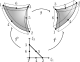
\includegraphics[width=.4\linewidth]{Figuras/Mapeamento.pdf}
    \\Fonte: Autoria Própria (\the\year).
    \label{fig:Mapeamento}
\end{figure}

Sendo assim, os parâmetros dependentes do espaço podem ser aproximados como:

\begin{subequations}
    \begin{align}
         & f_i^{m0}=x_i^m=X_i^aN_a(\xi_1,\xi_2)\text{,}                                            \\
         & f_i^{m1}=y_i^m=Y_i^aN_a(\xi_1,\xi_2)\text{,}                                            \\
         & f_i^0=x_i^m+v_i^0\text{,}                                                               \\
         & f_i^1=y_i^m+v_i^1\text{,}                                                               \\
         & v_i^0=\frac{h_0}{2}N_ a(\xi_1,\xi_2)(V^0)_i^a\xi_3\text{,}                              \\
         & v_i^1=\frac{h_0}{2}N_ a(\xi_1,\xi_2)(V^0)_i^a[\xi_3+\alpha(\xi_1,\xi_2)\xi_3^2]\text{,} \\
         & \alpha(\xi_1,\xi_2)=\Alpha^aN_a(\xi_1,\xi_2)\text{,}                                    \\
         & t_i=T_i^aN_a(\xi_1,\xi_2)\text{ e}                                                      \\
         & q_i=Q_i^aN_a(\xi_1,\xi_2)\text{,}
    \end{align}
\end{subequations}

\noindent em que $X_i^a$ representa a posição inicial de um nó $a$, $f_i^{m0}$ e $f_i^{m1}$ são as funções de mudança de configuração da superfície média $\Omega_\xi\to\Omega_0$ e $\Omega_\xi\to\Omega$, respectivamente, onde $\Omega_\xi$ é o espaço paramétrico e $\Omega$ é a configuração atual do contínuo, $v_i^0$ é o vetor unitário normal à superfície média, $v_i^1$ é o vetor generalizado na configuração atual, $h_0$ é a espessura inicial da casca, $N_a$ é a função de forma, $T_i^a$ é o valor de $t_i$ sobre o nó $a$, $Q_i^a$ é o valor de $q_i$ sobre o nó $a$ e $\alpha$ é uma variável inserida no problema, denominada como taxa de variação da espessura, cujo valor sobre o nó $a$ é $\Alpha^a$ \cite{sanches2013unconstrained,sanches2014fluid}.

Note que $\BB{f}(\BB{x},t)=\BB{f}^1((\BB{f}^0)^{-1},t)$, portanto é possível se obter o gradiente da função de mudança de configuração ($\BB{A}=\partial\BB{f}/\partial\BB{x}$) como $\BB{A}=\BB{A}^1\cdot(\BB{A}^0)^{-1}$, em que os valores de $\BB{A}^1$ são:

\begin{subequations}
    \begin{align}
         & A_{i1}^1=f_{i,1}^1=Y_i^aN_{a,1}+\frac{h_0}{2}\bigpar{(V^1)_i^aN_aA^bN_{b,1}\xi_3^2+(V^1)_i^aN_{a,1}(\xi_3+\Alpha^bN_b\xi_3^2)}\text{,}  \\
         & A_{i2}^1=f_{i,2}^1=Y_i^aN_{a,2}+\frac{h_0}{2}\bigpar{(V^1)_i^aN_aA^bN_{b,2}\xi_3^2+(V^1)_i^aN_{a,2}(\xi_3+\Alpha^bN_b\xi_3^2)}\text{ e} \\
         & A_{i3}^1=f_{i,3}^1=\frac{h_0}{2}(V^1)_i^aN_a\bigpar{1+2A^bN_b\xi_3}
    \end{align}
    \label{eq:CSD-A1}
\end{subequations}

\noindent e os valores de $\BB{A}^0$ são:

\begin{subequations}
    \begin{align}
         & A_{i1}^0=f_{i,1}^0=X_i^aN_{a,1}+\frac{h_0}{2}(V^0)_i^aN_{a,1}\xi_3\text{,}  \\
         & A_{i2}^0=f_{i,2}^0=X_i^aN_{a,2}+\frac{h_0}{2}(V^0)_i^aN_{a,2}\xi_3\text{ e} \\
         & A_{i3}^0=f_{i,3}^0=\frac{h_0}{2}(V^0)_i^aN_a\text{.}
    \end{align}
    \label{eq:CSD-A0}
\end{subequations}

Assim, considera-se o princípio da conservação da energia como:

\begin{equation}
    \delta\Pi=\der{\Pi_0}{g_i}\delta g_i=0\text{,}
\end{equation}

\noindent em que $\BB{g}$ representa o vetor que contém todos os graus de liberdade do problema.

Logo, precisa-se calcular a derivada de $\Pi_0$ em relação à $\BB{Y}$, $\BB{V}^1$ e $\BB{\Alpha}$. Dessa forma tem-se as seguintes derivadas:

\begin{subequations}
    \begin{equation}
        \begin{split}
            \der{\Pi_0}{Y_i^a}=&\der{\mathbb{U}}{Y_i^a}+
            \intDomi{\lambda_m\rho_0N_a\dot{y}_i}+
            \intDomi{\rho_0N_a\ddot{y}_i}-
            F_i^a-\\
            &\intFronti{N_at_i}
            -\intFronti{N_aq_i}=0\text{,}
        \end{split}
    \end{equation}
    \begin{equation}
        \begin{split}
            \der{\Pi_0}{(V^1)_i^a}=&\der{\mathbb{U}}{(V^1)_i^a}
            +\intDomi{\lambda_m\rho_0\frac{h_0}{2}N_a(\xi_3+\alpha\xi_3^2)\dot{y}_i}\\
            &+\intDomi{\rho_0\frac{h_0}{2}N_a(\xi_3+\alpha\xi_3^2)\ddot{y}_i}-
            \intFronti{q_i\frac{h_0}{2}N_a(\xi_3+\alpha\xi_3^2)}=0\text{,}
        \end{split}
    \end{equation}
    \begin{equation}
        \begin{split}
            \der{\Pi_0}{\Alpha^a}=&\der{\mathbb{U}}{\Alpha^a}
            +\intDomi{\lambda_m\rho_0\frac{h_0}{2}(V^1)_i^bN_aN_b\xi_3^2\dot{y}_i}\\
            &+\intDomi{\rho_0\frac{h_0}{2}N_aN_b(V^1)_i^b\xi_3^2\ddot{y}_i}-
            \intFronti{q_i\frac{h_0}{2}(V^1)_i^bN_aN_b\xi_3^2}=0\text{,}
        \end{split}
    \end{equation}
\end{subequations}

\noindent sendo possível definir um vetor resíduo $\BB{r}$ como:

\begin{equation}
    r_i^a(\BB{Y},\BB{V}^1,\BB{\Alpha})=(F^\mathrm{int})_i^a+(F^\mathrm{amort})_i^a+(F^\mathrm{inerc})_i^a-(F^\mathrm{c})_i^a-(F^\mathrm{nc})_i^a=0\text{,}
    \label{eq:CSD-g}
\end{equation}

\noindent sendo $\BB{Y}$, $\BB{V}^1$ e $\Alpha$ os vetores dos graus de liberdade nodais do elemento analisado:

\begin{subequations}
    \begin{align}
         & (F^\mathrm{int})_i^a=\intDomi{\der{u_e}{g_i^a}}=\intDomi{S_{kl}\der{\mathbb{E}_{kl}}{g_i^a}}\text{,}\label{eq:CSD-Fint} &  & \text{Forças internas}          \\
         & (F^\mathrm{amort})_i^a=\intDomi{\lambda_m\rho_0\der{y_j}{g_i^a}\dot{y}_j}\text{,}\label{eq:CSD-Famort}                  &  & \text{Forças de amortecimento}  \\
         & (F^\mathrm{inerc})_i^a=\intDomi{\rho_0\der{y_j}{g_i^a}\ddot{y}_j}\text{,}\label{eq:CSD-Finerc}                          &  & \text{Forças inerciais}         \\
         & (F^\mathrm{c})_i^a=F_j^b\der{Y_j^b}{g_i^a}+\intFronti{t_j\der{y_j^m}{g_i^a}}\text{ e}\label{eq:CSD-Fc}                  &  & \text{Forças conservativas}     \\
         & (F^\mathrm{nc})_i^a=\intFronti{q_j\der{y_j^m}{g_i^a}}\text{.}\label{eq:CSD-Fnc}                                           &  & \text{Forças não-conservativas}
    \end{align}
    \label{eq:CSD-F}
\end{subequations}

Portanto o problema ser resolvido é descrito como: determinar $\BB{Y}$, $\BB{V}^1$ e $\BB{\Alpha}$ tais que $\BB{r}(\BB{Y},\BB{V}^1,\BB{\Alpha})=\BB{0}$.

Como é possível verificar, o cálculo de $\BB{r}$ é dependente não somente dos parâmetros nodais, mas também das derivadas de primeira e segunda ordem desses parâmetros. Sendo assim, se faz necessária a consideração de um integrador temporal, o qual será utilizado o integrador temporal de Newmark, devido à capacidade de respeitar a conservação de momento linear para $\gamma=1/2$ e apresentando bons resultados para modelagem de elementos de casca, conforme apresentado por \citeonline{sanches2013unconstrained}.

A aproximação realizada pelo integrador de Newmark é dada por:

\begin{subequations}
    \begin{equation}
        g_i^{n+1}=g_i^n+\dot{g}_i^n\Delta t+\Delta t^2\bigpar{\bigpar{\frac{1}{2}-\beta}\ddot{g}_i^n+\beta\ddot{g}_i^{n+1}}\text{ e}
    \end{equation}
    \begin{equation}
        \dot{g}_i^{n+1}=\dot{g}_i^n+\Delta t(1-\gamma)\ddot{g}_i^n+\gamma\ddot{g}_i^{n+1}\Delta t\text{,}
    \end{equation}
\end{subequations}

\noindent sendo o superíndice $n$ e $n+1$ a indicação do passo de tempo analisado ($t_n$ e $t_{n+1}$), $\Delta t$ o intervalo de tempo discretizado e $\beta$ e $\gamma$ parâmetros livres, que devem ser escolhidos de forma a garantir a convergência do método, sendo arbitrados valores de $\beta=1/4$ e $\gamma=1/2$, garantindo a estabilidade incondicional do método \cite{LINDFIELD2019239}.

Isolando-se os termos incógnitos em função de parâmetros não derivados no tempo em $n+1$ e daqueles já conhecidos tem-se:

\begin{subequations}
    \begin{align}
         & \ddot{g}_i^{n+1}=\frac{g_i^{n+1}}{\beta\Delta t^2}-Q_i^n                                \\
         & \dot{g}_i^{n+1}=\frac{\gamma}{\beta\Delta t}g_i^{n+1}+R_i^n-\gamma\Delta tQ_i^n\text{,}
    \end{align}
    \label{eq:CSD-Newmark2}
\end{subequations}

\noindent em que:

\begin{subequations}
    \begin{align}
         & Q_i^n=\frac{g_i^n}{\beta\Delta t^2}+\frac{\dot{g}_i^n}{\beta\Delta t}+\bigpar{\frac{1}{2\beta}-1}\ddot{g}_i^n \\
         & R_i^n=\dot{g}_i^n+\Delta t(1-\gamma)\ddot{g}_i^n\text{.}
    \end{align}
    \label{eq:CSD-QnRn}
\end{subequations}

Já para procurar valores de $\BB{g}$ que anulem $\BB{r}$, utiliza-se o Método de Newton-Raphson, o qual parte da aproximação por série de Taylor truncada no termo de primeira ordem:

\begin{equation}
    \begin{split}
        &\BB{r}(\BB{g}+\Delta\BB{g})=\BB{r}(\BB{g})+\apderp{\BB{r}}{\BB{g}}{\BB{g}}\Delta\BB{g}=\\
        &\BB{r}(\BB{Y},\BB{V}^1,\BB{\Alpha})+\apderp{\BB{r}}{\BB{Y}}{\BB{Y}}\Delta\BB{Y}+\apderp{\BB{r}}{\BB{V}^1}{\BB{V}^1}\Delta\BB{V}^1+\apderp{\BB{r}}{\BB{\Alpha}}{\BB{\Alpha}}\Delta\BB{\Alpha}=\BB{0}\text{.}
    \end{split}
\end{equation}

\noindent Dessa forma, necessita-se do cálculo de uma matriz Hessiana ($H_{ij}^{ab}$):

\begin{equation}
    H_{ij}^{ab}=\frac{\partial^2\Pi_0}{\partial g_j^b\partial g_i^a}=\der{r_i^a}{g_j^b}\text{.}
\end{equation}

Substituindo-se as derivadas temporais da aproximação de Newmark em $\BB{r}$ e realizando as devidas simplificações, obtém-se:

\begin{equation}
    H_{ij}^{ab}=(H^\text{est})_{ij}^{ab}+\frac{\gamma C_{ij}^{ab}}{\beta\Delta t}+\frac{M_{ij}^{ab}}{\beta\Delta t^2}+\intDom{\rho_0(\lambda_m\dot{y}_k+\ddot{y}_k)\Dder{y_k}{g_j^b}{g_i^a}}\text{,}
    \label{eq:CSD-Hijab}
\end{equation}

\noindent sendo $(H^\text{est})_{ij}^{ab}$ a matriz hessiana estática elementar, $M_{ij}^{ab}$ a matriz de massa e $C_{ij}^{ab}$ a matriz de amortecimento, dadas por:

\begin{subequations}
    \begin{align}
         & (H^\text{est})_{ij}^{ab}=\Dder{\mathbb{U}}{g_j^b}{g_i^a}=\intDomi{\bigpar{\der{S_{kl}}{g_j^b}\der{\mathbb{E}_{kl}}{g_i^a}+S_{kl}\Dder{\mathbb{E}_{kl}}{g_i^a}{g_j^b}}} \\
         & C_{ij}^{ab}=\intDomi{\lambda_m\rho_0\der{y_k}{g_i^a}\der{y_k}{g_j^b}}\text{ e}                                                                                         \\
         & M_{ij}^{ab}=\intDomi{\rho_0\der{y_k}{g_i^a}\der{y_k}{g_j^b}}\text{.}
    \end{align}
    \label{eq:CSD-HMC}
\end{subequations}

\noindent também observa-se que a derivada mista de $y_k$ em relação a $g_i^a$ e $g_j^b$ possuirá valores não-nulos apenas quando for derivada de forma cruzada em relação a $V^1$ e $\Alpha$.

Com isso, encontra-se um vetor de correções dos parâmetros nodais ($\Delta\BB{g}$) como a solução do sistema:

\begin{equation}
    H_{ij}\Delta g_j=-r_i\text{,}
\end{equation}

\noindent tendo como critério de parada a medida do erro:

\begin{equation}
    \frac{\norm{\Delta\BB{Y}}}{\norm{\BB{X}}}\leq\text{tol,}
    \label{eq:CSD-erro}
\end{equation}

\noindent em que $\BB{X}$ o vetor de posições nodais iniciais e tol uma tolerância admitida.

%==================================================================================================
\subsubsection{Procedimento Computacional} \label{MEFP-Comp}
%==================================================================================================

Para a implementação computacional realizou-se uma integração em $\Omega_0$ e $\Gamma_0$ segundo a quadratura de hammer \cite{hammer1956numerical}, sendo a malha gerada automaticamente via comunicação direta do algoritmo com o \textit{Gmsh} e o procedimento paralelizado utilizando o protocolo MPI presente na biblioteca PETSc. Demais informações relevantes à implementação computacional são descritas detalhadamente no capítulo \ref{MetodologiaCronograma}.

O algoritmo \ref{alg:MEF-casca} apresentado na forma de pseudocódigo exemplifica o código implementado.

\begin{algorithm}[h!]
    \caption{Algoritmo utilizado para o cálculo das posições nodais.}
    \label{alg:MEF-casca}
    \KwResult{Vetor global de parâmetros nodais}
    $\BB{Y}\gets\BB{X}$\;
    \For{$t_i\gets 0$ \KwTo $t_f$}{
    Calcular $Q^n$ e $R^n$ (Eq. \ref{eq:CSD-QnRn})\;
    \ForEach{\textnormal{passo de carga}}{
    \tcp{Cálculo das forças externas}
    \ForEach{\textnormal{elemento}}{
    \ForEach{\textnormal{ponto de Hammer }$i_h$}{
    Calcular $\BB{A}^0_{2\times 2}$ e $J_0=\det{(A^0)}$\;
    \ForEach{\textnormal{Nó $a$ do elemento na direção $i$}}{
        Calcular $\BB{F}^c$ e $\BB{F}^{nc}$ (Eq. \ref{eq:CSD-Fc} e \ref{eq:CSD-Fnc})\;
        Somar a contribuição no vetor global: $((F^c)_i^a+(F^{nc})_i^a)\cdot J_0\cdot w_{i_h}$\;
    }
    }
    }
    Somar a contribuição das forças concentradas no vetor global\;
    \While{erro>tol}{
    \ForEach{\textnormal{elemento}}{
    \ForEach{\textnormal{ponto de Hammer }$i_h$}{
    Calcular $\BB{A}^0_{3\times 3}$ (Eq. \ref{eq:CSD-A0}), $J_0=\det{(A^0)}$, $(\BB{A}^0)^{-1}_{3\times 3}$ e $\BB{A}^1_{3\times 3}$ (Eq. \ref{eq:CSD-A1})\;
    Calcular $\BB{A}_{3\times 3}=\BB{A}^1\cdot(\BB{A}^0)^{-1}$\;
    Calcular $\BB{C}_{3\times 3}=\BB{A}^T\cdot\BB{A}$\;
    Calcular $\mathbb{E}_{3\times 3}$ (Eq. \ref{eq:CSD-DefGreenLagr})\;
    Calcular $\BB{S}_{3\times 3}$ (Eq. \ref{eq:CSD-S})\;
    \ForEach{\textnormal{Nó $a$ do elemento na direção $i$}}{
        Calcular $r_i^a$ (Eq. \ref{eq:CSD-g} e \ref{eq:CSD-Fint} a \ref{eq:CSD-Finerc})\;
        Somar a contribuição no vetor global: $r_i^a\cdot J_0\cdot w_{i_h}$\;
        \ForEach{\textnormal{Nó $b$ do elemento na direção $j$}}{
            Calcular $H_{ij}^{ab}$ (Eq. \ref{eq:CSD-Hijab} e \ref{eq:CSD-HMC})\;
            Somar a contribuição na matriz global: $H_{ij}^{ab}\cdot J_0\cdot w_{ih}$\;
        }
    }
    }
    }
    Resolver o sistema global: $\BB{H}\cdot\Delta\BB{g}=-\BB{r}$\;
    Atualizar os parâmetros nodais: $\BB{g}\gets\BB{g}+\Delta\BB{g}$\;
    Atualizar derivadas temporais (Eq. \ref{eq:CSD-Newmark2})\;
    Cálculo do erro via \ref{eq:CSD-erro}\;
    }
    }
    Atualização dos valores passados\;
    }
\end{algorithm}

%==================================================================================================
\subsubsection{Exemplos de Verificação} \label{MEFP-Ex}
%==================================================================================================

Na presente seção serão apresentadas algumas simulações realizadas utilizando o procedimento supracitado, com a finalidade de validar o código utilizado.

%==================================================================================================
\subsubsubsection{\textit{Scordelis-Lo roof}}
%==================================================================================================

O primeiro exemplo simulado trata-se de um problema comumente encontrado para problemas de cascas, denominado de \textit{Scordelis-Lo roof}, conforme ilustrado na Figura \ref{fig:scordelis}. Esse exemplo se caracteriza por uma cobertura curva sujeita a um carregamento gravitacional $q$, distribuído por unidade de área, na direção $x_3$ para baixo. Os parâmetros geométricos são dados por: comprimento $L=50$, raio de curvatura $R=25$, espessura $t=0,25$ e ângulo $\theta=40^\circ$. O valor da carga aplicada é $q=90$. O material que constitui a cobertura possui módulo de Young $E=4,32\times10^8$ e Poisson nulo. As extremidades estão presas por um diafragma rígido ($u_1=u_3=0$). Os resultados são comparados com os obtidos por \citeonline{BELYTSCHKO1985221,ZHOU2022108568,CHAUDINH2023110222}, os quais apontam que o deslocamento vertical do nó $A$ é de 0,3024.

\begin{figure}[h!]
    \centering
    \caption{Problema de \textit{Scordelis-Lo roof}.}
    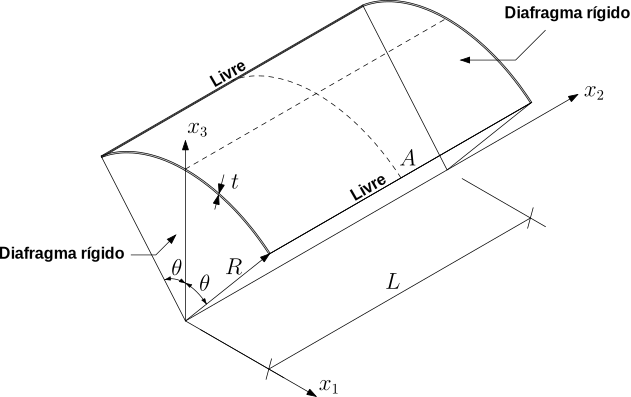
\includegraphics[width=0.75\linewidth]{Figuras/scordelis/scordelis_lo.pdf}
    \\Fonte: Autoria Própria (\the\year).
    \label{fig:scordelis}
\end{figure}

Para a simulação do problema aproveitou-se da simetria da cobertura, o que possibilitou a modelagem de apenas um quarto do problema. Assim utilizou-se uma malha estruturada com orientação à esquerda contendo 552 elementos triangulares de aproximação quadrática, resultando em 7987 graus de liberdade. A malha é apresentada na Figura \ref{fig:scordelis-mesh}. As faces laterais observadas na malha foram criadas por conta da forma de construção da aresta circular da cobertura, sendo atribuídos $E=\nu=0$ para os elementos dessas faces. O problema foi considerado em pequenos deslocamentos e deformações, ou seja, utilizou-se somente uma iteração de Newton-Raphson.

\begin{figure}[h!]
    \centering
    \caption{Malha utilizada na simulação de \textit{Scordelis-Lo roof}.}
    \begin{subfigure}{0.4\textwidth}
    \includegraphics[width=\linewidth]{Figuras/scordelis/malha1.png}
    \caption{Perspectiva isométrica.}
    \end{subfigure}
    \begin{subfigure}{0.4\textwidth}
    \includegraphics[width=\linewidth]{Figuras/scordelis/malha2.png}
    \caption{Vista superior.}
    \end{subfigure}
    \\Fonte: Autoria Própria (\the\year).
    \label{fig:scordelis-mesh}
\end{figure}

Dessa forma, chegou-se a um deslocamento de 0,3008 nos cálculos realizados, representando um desvio de 0,5291\% em relação à referência. Também analisou-se o resultado com aquele obtido pelo \textit{software} ANSYS, o qual retornou um deslocamento de 0,3020. Assim o desvio relativo do resultado calculado com o do ANSYS é de 0,3973\%. A Figura \ref{fig:scordelis-displ} apresenta o campo de deslocamentos obtido para um quadrante da cobertura.

\begin{figure}[h!]
    \centering
    \caption{Campos de deslocamentos obtido na simulação de \textit{Scordelis-Lo roof}.}
    \begin{subfigure}{0.075\textwidth}
    \includegraphics[width=\linewidth]{Figuras/scordelis/eixos.png}
    \end{subfigure}
    \begin{subfigure}{0.4\textwidth}
    \includegraphics[width=\linewidth]{Figuras/scordelis/ux.png}
    \end{subfigure}
    \begin{subfigure}{0.4\textwidth}
    \includegraphics[width=\linewidth]{Figuras/scordelis/uy.png}
    \end{subfigure}
    \begin{subfigure}{0.4\textwidth}
    \includegraphics[width=\linewidth]{Figuras/scordelis/uz.png}
    \end{subfigure}
    \\Fonte: Autoria Própria (\the\year).
    \label{fig:scordelis-displ}
\end{figure}

Assim, observa-se que tais campos estão muito semelhantes aos apresentados por \citeonline{ZHOU2022108568}, sendo satisfatoriamente verificada a análise realizada.

%==================================================================================================
\subsubsubsection{Cilindro biengastado}
%==================================================================================================

Outro problema comum considera um cilindro sujeito a duas cargas concentradas diametralmente opostas, conforme visto na Figura \ref{fig:cylinder-shell}. As dimensões do problema são: comprimento $L=600$, raio $R=300$ e espessura $t=3$. A carga aplicada é $P=1$. O material que constitui o cilindro possui módulo de elasticidade $E=3\times10^6$ e coeficiente de Poisson $\nu=0,3$. Ambas as extremidades do cilindro estão vinculadas a um diafragma rígido, ou seja, $u_1=u_3=\phi_2=0$. O resultado de referência adotado é de um deslocamento radial de $1,8248\times10^{-5}$ no ponto de aplicação da carga \cite{BELYTSCHKO1985221,CHAUDINH2023110222,ZHOU2022108568}.

\begin{figure}[h!]
    \centering
    \caption{Cilindro submetido a forças concentradas.}
    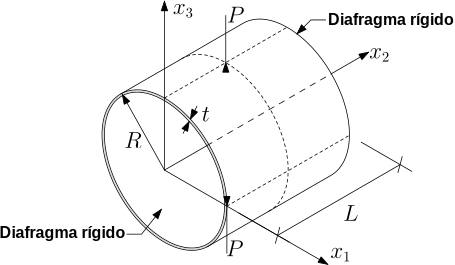
\includegraphics[width=0.65\linewidth]{Figuras/cylinder-shell/cylinder.pdf}
    \\Fonte: Autoria Própria (\the\year).
    \label{fig:cylinder-shell}
\end{figure}

Pelo fato do problema apresentar simetria, foi estudado somente um octante do problema. Assim utilizou-se uma malha estruturada para a direita contendo 1232 elementos triangulares de aproximação quadrática, contando com um total de 39823 graus de liberdade. A malha utilizada é observada na Figura \ref{fig:cylinder-shell-mesh}. As faces laterais devido ao processo de geração da aresta circular possuem $E=\nu=0$. Na simulação adotou-se uma aproximação linear da solução.

\begin{figure}[h!]
    \centering
    \caption{Malha utilizada na simulação de \textit{Scordelis-Lo roof}.}
    \begin{subfigure}{0.3\textwidth}
    \includegraphics[width=\linewidth]{Figuras/cylinder-shell/mesh1.png}
    \caption{Perspectiva isométrica.}
    \end{subfigure}
    \begin{subfigure}{0.3\textwidth}
    \includegraphics[width=\linewidth]{Figuras/cylinder-shell/mesh2}
    \caption{Vista superior.}
    \end{subfigure}
    \\Fonte: Autoria Própria (\the\year).
    \label{fig:cylinder-shell-mesh}
\end{figure}

O resultado obtido foi de um deslocamento radial de $1,8485\times10^{-5}$, tendo, portanto, um desvio relativo de $1,2988\%$ em relação à referência. Também se comparou o resultado obtido com relação à uma simulação feita no \textit{software} ANSYS, a qual resultou em um deslocamento de $1,8504\times10^{-5}$. Logo o desvio do resultado calculado com o apresentado pelo ANSYS foi de $0,1027\%$. Os campos de deslocamentos obtidos são apresentados na Figura \ref{fig:cylinder-shell-disp}.

\begin{figure}[h!]
    \centering
    \caption{Campos de deslocamentos obtido na simulação de cilindro.}
    \begin{subfigure}{0.075\textwidth}
    \includegraphics[width=\linewidth]{Figuras/cylinder-shell/eixos.png}
    \end{subfigure}
    \begin{subfigure}{0.3\textwidth}
    \includegraphics[width=\linewidth]{Figuras/cylinder-shell/ux.png}
    \end{subfigure}
    \begin{subfigure}{0.3\textwidth}
    \includegraphics[width=\linewidth]{Figuras/cylinder-shell/uy.png}
    \end{subfigure}
    \begin{subfigure}{0.3\textwidth}
    \includegraphics[width=\linewidth]{Figuras/cylinder-shell/uz.png}
    \end{subfigure}
    \\Fonte: Autoria Própria (\the\year).
    \label{fig:cylinder-shell-disp}
\end{figure}

Verifica-se, então, que os resultados dos campos de deslocamentos são muito próximos aos obtidos por \citeonline{ZHOU2022108568}.

Também realizou-se uma análise quanto à convergência da malha nos problemas de \textit{Scordelis-Lo roof} e do cilindro biengastado, onde dividiu-se as arestas do problema em $N$ partes. As Tabelas \ref{tab:scordelis-sol} e \ref{tab:cylinder-shell-sol} apresentam os resultados obtidos, sendo os valores dos desvios relativos ilustrados na Figura \ref{fig:shell-static-sol}.

\begin{table}[h!]
    \centering
    \caption{Análise da convergência da malha para o problema de \textit{Scordelis-Lo roof}.}
    \begin{tabular}{ccccc}
        \hline
        $N$  & Número de elementos & Graus de liberdade & Calculado & Desvio relativo \\\hline
        5    & 64                  & 1001               & 0,2115    & -30,060\%       \\
        6    & 88                  & 1351               & 0,2361    & -21,925\%       \\
        7    & 11                  & 1757               & 0,2638    & -12,765\%       \\
        8    & 148                 & 2219               & 0,2726    & -9,854\%        \\
        9    & 184                 & 2737               & 0,2824    & -6,614\%        \\
        10   & 224                 & 3311               & 0,2863    & -5,324\%        \\
        11   & 268                 & 3941               & 0,2893    & -4,332\%        \\
        12   & 316                 & 4627               & 0,2925    & -3,274\%        \\
        13   & 368                 & 5369               & 0,2954    & -2,325\%        \\
        14   & 424                 & 6167               & 0,2970    & -1,786\%        \\
        15   & 484                 & 7021               & 0,2978    & -1,521\%        \\
        16   & 552                 & 7987               & 0,3008    & -0,529\%        \\\hline
    \end{tabular}
    \\Fonte:Autoria Própria (\the\year).
    \label{tab:scordelis-sol}
\end{table}

\begin{table}[h!]
    \centering
    \caption{Análise da convergência da malha para o problema do cilindro biengastado.}
    \begin{tabular}{ccccc}
        \hline
        $N$  & Número de elementos & Graus de liberdade & Calculado  & Desvio relativo \\\hline
        5    & 124                 & 4228               & 1,4147E-05 & -22,474\%       \\
        6    & 184                 & 6181               & 1,5710E-05 & -13,908\%       \\
        7    & 240                 & 8008               & 1,6630E-05 & -8,867\%        \\
        8    & 316                 & 10465              & 1,7228E-05 & -5,590\%        \\
        9    & 396                 & 13048              & 1,7636E-05 & -3,354\%        \\
        10   & 488                 & 16009              & 1,7863E-05 & -2,110\%        \\
        11   & 572                 & 18718              & 1,7993E-05 & -1,397\%        \\
        12   & 692                 & 22561              & 1,8210E-05 & -0,208\%        \\
        13   & 808                 & 26278              & 1,8241E-05 & -0,038\%        \\
        14   & 940                 & 30499              & 1,8331E-05 & 0,455\%         \\
        15   & 1062                & 34405              & 1,8436E-05 & 1,031\%         \\
        16   & 1232                & 39823              & 1,8485E-05 & 1,299\%         \\\hline
    \end{tabular}
    \\Fonte:Autoria Própria (\the\year).
    \label{tab:cylinder-shell-sol}
\end{table}

\begin{figure}[h!]
    \centering
    \caption{Valores dos desvios em ambos os problemas estáticos analisados.}
    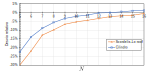
\includegraphics[width=0.75\linewidth]{Figuras/cylinder-shell/static-sol.pdf}
    \\Fonte: Autoria Própria (\the\year).
    \label{fig:shell-static-sol}
\end{figure}

%==================================================================================================
\subsubsubsection{Viga engastada em problema dinâmico}
%==================================================================================================

Para verificação do código implementado em problemas dinâmicos, estudou-se  primeiramente o comportamento de uma viga engastada em uma de suas extremidades e sujeita a uma carga $P$ aplicada na extremidade oposta, conforme ilustrado na Figura \ref{fig:viga1}. As dimensões da viga são: comprimento $L=60$ dm, altura $h=3$ dm e largura $b=1$ dm. A força aplicada possui intensidade $P=1,25\times10^{-4}$ Mg$\cdot$dm/(ms)² $H(t)$, sendo $H(t)$ a função de Heavside. O material que compõe a viga possui módulo de Young $E=20$ Mg/[dm$\cdot$(ms)²], coeficiente de Poisson nulo e massa específica $\rho=7\times10^{-3}$ Mg/dm³. O intervalo de tempo analisado foi $t\in[0;675]$ ms discretizado em passos de tempo $\Delta t=0,3377$. A malha de elementos finitos utilizada conta com 32 elementos triangulares de aproximação quadrática, com um total de 693 graus de liberdade, a qual pode ser observada na Figura \ref{fig:viga1-mesh}.

\begin{figure}[h!]
    \centering
    \caption{Desenho esquemático da viga simulada.}
    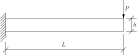
\includegraphics[width=0.5\linewidth]{Figuras/vigas/viga1.pdf}
    \\Fonte: Autoria Própria (\the\year).
    \label{fig:viga1}
\end{figure}

\begin{figure}[h!]
    \centering
    \caption{Malha utilizada na simulação da viga.}
    \includegraphics[width=\linewidth]{Figuras/vigas/mesh1.png}
    \\Fonte: Autoria Própria (\the\year).
    \label{fig:viga1-mesh}
\end{figure}

A modelagem realizada considerou a altura $H$ como a espessura do elemento de casca, sendo a força atuante nessa mesma direção. Assim, observou-se o deslocamento vertical no ponto de aplicação da força. Os resultados obtidos foram comparados com aqueles alcançados a partir de uma modelagem no \textit{software} ANSYS utilizando elementos sólidos 183. a Figura \ref{fig:res-viga1} apresenta os resultados calculados.

\begin{figure}[h!]
    \centering
    \caption{Deslocamento vertical no ponto de aplicação da força ao longo do tempo.}
    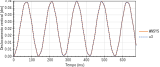
\includegraphics[width=\linewidth]{Figuras/vigas/res1.pdf}
    \\Fonte: Autoria Própria (\the\year).
    \label{fig:res-viga1}
\end{figure}

Observa-se nesse caso uma boa concordância entre os resultados apresentados pelo ANSYS e os obtidos pelo código desenvolvido, sendo verificada a eficácia nesse exemplo.

Outro exemplo trata-se de uma viga biengastada com uma carga aplicada em seu centro, conforme mostrado na Figura \ref{fig:viga2}. Nesse exemplo considerou-se um comprimento $L=20$ in, com seção transversal de $b\times h=1,0\times0,125$ in². O material que constitui a viga possui módulo de Young $E=3\times10^{7}$ lb/in², coeficiente de Poisson nulo e massa específica de $\rho=2,6\times10^{-4}$ lb$\cdot$s²/in$^4$. A força aplicada foi de $P=640$ lb constante durante todo o período de análise, de $t\in[0;5]$ ms, o qual foi discretizado em passos de tempo de $\Delta t=25\ \mu$ s. A malha de elementos finitos (Figura \ref{fig:viga2-mesh}) possui 132 elementos triangulares de aproximação quadrática, totalizando 2331 graus de liberdade. A espessura do elemento de casca foi considerado como a direção da altura $H$ da viga.

\begin{figure}[h!]
    \centering
    \caption{Desenho esquemático da viga biengastada simulada.}
    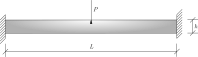
\includegraphics[width=0.6\linewidth]{Figuras/vigas/viga2.pdf}
    \\Fonte: Autoria Própria (\the\year).
    \label{fig:viga2}
\end{figure}

\begin{figure}[h!]
    \centering
    \caption{Malha utilizada na simulação da viga biengastada.}
    \includegraphics[width=\linewidth]{Figuras/vigas/mesh2.png}
    \\Fonte: Autoria Própria (\the\year).
    \label{fig:viga2-mesh}
\end{figure}

Os resultados calculados foram comparados com os apresentados pelo ANSYS, a partir do elemento 183, e por \cite{mondkar1977ansa}. A Figura \ref{fig:res-viga2} exibe os resultados obtidos.

\begin{figure}[h!]
    \centering
    \caption{Deslocamento vertical no centro da viga biengastada ao longo do tempo.}
    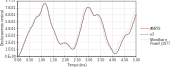
\includegraphics[width=\linewidth]{Figuras/vigas/res2.pdf}
    \\Fonte: Autoria Própria (\the\year).
    \label{fig:res-viga2}
\end{figure}

Verifica-se uma boa concordância entre os resultados obtidos pela análise por ambos os valores de referência, sendo assim, averiguada a eficácia do código nesse exemplo.